\chapter{Research}\label{chap:research}

%---------------------------------------------------------------
\section{Operating System: FreeRTOS}

%...........................................
\subsection{Overview}

% Quick overview of the system: Free, open source, GP Licence, light-weight

\hspace{15mm}FreeRTOS is a light-weight and real-time\footnote{A system that should fit to time constraints.} operating system suitable for embedded devices. It is distributed under the GPL\footnote{General public licence is used for free and open source software.} even then with certain exceptions: a developer is required to maintain the kernel as open source, whereas he could remain closed source his applications.

\begin{figure}[h]
  \centering
  
\includegraphics[scale=0.125]{images/freertos.jpg}
  \caption{FreeRTOS logo}
\end{figure}

The FreeRTOS source code is tiny and simple, thus it is really easy to port. It is mostly written in C and assembly. The kernel has been ported to around thirty micro-controllers.

The system kernel consists of three common main files (\textit{list.c}, \textit{queue.c} and \textit{tasks.c}) and at least one specific to a particular micro-controller (\textit{port.c}).



%...........................................
\subsection{Real-Time System}

% Kernel mechanism: priorities and scheduling
\hspace{15mm}One of the main feature provided by FreeRTOS is the way the system performs threads. All tasks are scheduled depending on their priority and sorted according to a round-robin algorithm.

Every files which manage tasks should include the FreeRTOS header \textit{task.h} in order to use the appropriate functions.

A task can be defined as follows and should be of endless loop style:\clearpage
\begin{lstlisting}
void vMyTask (void * pvParameters)
{
	for(;;)
	{
		/* Task code content */
	}
}
\end{lstlisting}

The FreeRTOS thread API\footnote{An Application Programming Interface is a set of routines or functions given by a library.} allows to manage tasks. For instance, to create or delete them:
\begin{lstlisting}
xTaskHandle xHandle;

xTaskCreate( vMyTask, "NAME", STACK_SIZE, &parameters, tskIDLE_PRIORITY, &xHandle );
vTaskDelete( xHandle );
\end{lstlisting}
The \cfunction{xTaskHandle} element allows to keep a reference to the task that can be then used by other functions

Depending on its presence or its position in the queue, a task can take different states:
\begin{itemize}
\item \textit{Ready}: the task is ready to run but it is not currently executing because another task is running. From this state, it might become \textit{Suspended} or \textit{Running}.
\item \textit{Running}: the task is currently executing. From this state, it might become \textit{Blocked}, \textit{Ready} or \textit{Suspended}.
\item \textit{Blocked}: the task is not available for scheduling until a defined delay period. From this state, it might become \textit{Suspended} or \textit{Ready}.
\item \textit{Suspend}: the task is not available for scheduling without any timeout. From this state, it might become \textit{Ready}.
\end{itemize}
These states can be changed using the appropriate functions from the API, for instance:
\begin{lstlisting}
/* To suspend a specific task */
vTaskSuspend( xHandle );

/* To resume a suspended task */
vTaskResume( xHandle );

/* To raise a task priority */
vTaskPrioritySet( xHandle, tskIDLE_PRIORITY + 1 );
\end{lstlisting}


%...........................................
\subsection{POSIX simulator}

\hspace{15mm}To develop and test demo tasks in order to get knowledge about FreeRTOS, I worked with a simulator. This is a ported version of the operating system that allows an embedded application to be simulated on a computer running another system.

As I'm a Linux user, so I chose the POSIX simulator. This simulator consist of a set of files representing the kernel and some demo applications which can all be compiled using GCC\footnote{GNU Compiler Collection is a compiler system which can compile several programming languages including C and C++.}.

My first attempts to use the simulator were complicated by some undefined references issues at the compilation which came from my operating system. I did managed to fix the problem thanks to my supervisor Jo\~{a}o. At this point, I have been able to compile the simulator and to play with the demo applications and even create my own one.



%---------------------------------------------------------------
\section{Twitter authentication: OAuth protocol}

%...........................................
\subsection{Overview}

% Common authentication mechanism: token, secret key system, include graphic representations

\begin{figure}[h]
  \centering
  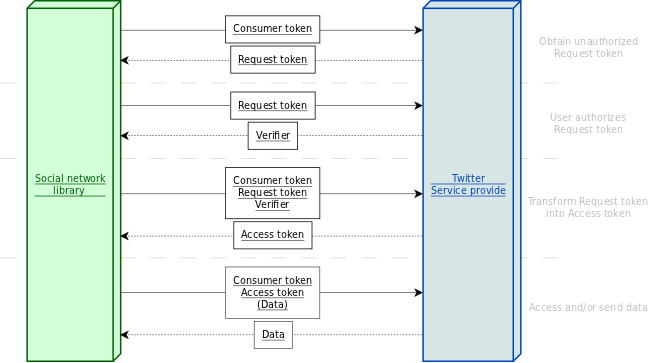
\includegraphics[scale=0.75]{images/oauth.png}
  \caption{OAuth protocol: communication process}
\end{figure}

\clearpage

OAuth is the secured protocol used by Twitter to allows developers to access and share data from a third-party application. The authentication process is based on the public and private key system. Each step of the process (from the authentication to the data access) is represented by a granted token. The authentication consists three different tokens:
\begin{itemize}
\item The \textit{Consumer token} is provided by the Twitter developers website at the application referencing.
\item The \textit{Request token} is given by the service provider as a temporary token.
\item The \textit{Access token} is given as a proof of authenticity that must be use to access and share data.
\end{itemize}


%...........................................
\subsection{Existing library in C}

% Downloaded and tested library: samples hard to understand, idea: create a simple-to-use library layer

\hspace{15mm}The Twitter developers documentation provides several implementations of OAuth protocol in many languages including C++, Java or Python, but for some reason not in C. However, I found a tiny C library under GPL, written by Robin Gareus and called \textit{liboauth}. His repository gives few examples, thus it was easy to get to know how to use it.

Basically, this library provides a set of functions to encode parameters according to OAuth specifications and to implement the protocol using HTTP requests (\textit{GET} and \textit{POST} methods). For instance, these functions could be used useful to perform the granting access rights: \cfunction{oauth\_sign\_url2()}, \cfunction{oauth\_http\_get()}, \cfunction{oauth\_http\_post()}. However, the whole Twitter authentication process is really complex and could be packaged as only one main routine.


%...........................................
\subsection{Register an application on Twitter}

% Way and proprieties of the registered application

\hspace{15mm}The first step is the account registration: I created a personal account which is the same no matter I use Twitter as a simple user sending tweets and following profiles, or as a developer creating applications using the API features.

Then, I registered a new application in the Twitter developers website to get the first required token to use the Twitter API via OAuth. The main informations are the name of the application and the access level: read and/or write which means that the application will be allowed to receive and/or send tweets.

At the end of the process, Twitter gives the \textit{Consumer token} (a set of a public and a private key) and also the useful URL to send requests. These URL are static so they might be stored into the main file that gather the whole authentication. 

\clearpage
\begin{figure}[h]
  \centering
  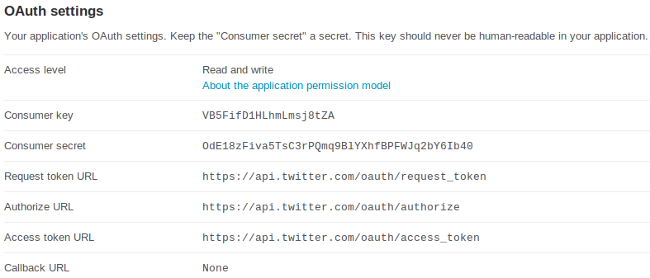
\includegraphics[scale=0.75]{images/register.png}
  \caption{Application informations from Twitter developers website}
\end{figure}


%...........................................
\subsection{Required libraries}

% libcurl: overview and it's seem hard to adapt to FreeRTOS, idea: create a very simple HTTP request library)
% OpenSSL: overview and it's seem hard to adapt to FreeRTOS, idea)

The liboauth required two libraries: \textbf{OpenSSL} and \textbf{libcurl}, thereby to build and library that could communicate with Twitter from an embedded device, these library must be ported and included.

OpenSSL is a open source library implementing the \textit{Secure Sockets Layer} and the \textit{Transport Layer Security} protocols and including several encryption algorithms. Libcurl is a library that allows to perform several kind of requests including FTP, IMAP, HTTP and HTTPS.

These two libraries are free open source and portable. As they could be compiled to be used with an embedded device, they are suitable for my project.

I downloaded both of them and I checked the source code. I even tried to quickly port and compile them to the FreeRTOS POSIX simulator, but without success. The investigation about how to fix the compilation issues should be put aside until the library fully works on the simulator.


\clearpage